% This must be in the first 5 lines to tell arXiv to use pdfLaTeX, which is strongly recommended.
\pdfoutput=1
% In particular, the hyperref package requires pdfLaTeX in order to break URLs across lines.

\documentclass[11pt]{article}

% Remove the "review" option to generate the final version.
\usepackage[]{acl}

% Standard package includes
\usepackage{times}
\usepackage{latexsym}

% For proper rendering and hyphenation of words containing Latin characters (including in bib files)
\usepackage[T1]{fontenc}
% For Vietnamese characters
% \usepackage[T5]{fontenc}
% See https://www.latex-project.org/help/documentation/encguide.pdf for other character sets

% This assumes your files are encoded as UTF8
\usepackage[utf8]{inputenc}

% This is not strictly necessary, and may be commented out,
% but it will improve the layout of the manuscript,
% and will typically save some space.
\usepackage{microtype}

% If the title and author information does not fit in the area allocated, uncomment the following
%
%\setlength\titlebox{<dim>}
%
% and set <dim> to something 5cm or larger.

\title{Health Risk Prediction Using Machine Learning
Across Heterogeneous Patient Populations}

% Author information can be set in various styles:
% For several authors from the same institution:
% \author{Author 1 \and ... \and Author n \\
%         Address line \\ ... \\ Address line}
% if the names do not fit well on one line use
%         Author 1 \\ {\bf Author 2} \\ ... \\ {\bf Author n} \\
% For authors from different institutions:
% \author{Author 1 \\ Address line \\  ... \\ Address line
%         \And  ... \And
%         Author n \\ Address line \\ ... \\ Address line}
% To start a seperate ``row'' of authors use \AND, as in
% \author{Author 1 \\ Address line \\  ... \\ Address line
%         \AND
%         Author 2 \\ Address line \\ ... \\ Address line \And
%         Author 3 \\ Address line \\ ... \\ Address line}

\author{Hams Aljohanu \\
  COE. Computer Science (AI) \\
  \texttt{S20106833} \\\And
  Ghala Alghamdi \\
  COE. Computer Science (AI)  \\  
  \texttt{S23108212} \\\And
  Hiba Amanulla  \\
  COE. Computer Science (AI) \\  
  \texttt{S23108227}
}
\usepackage{graphicx}
\begin{document}
\maketitle
\begin{abstract}
This project focuses on predicting hospital mortality for ICU patients using machine learning. The data used is the eICU Collaborative Research Database (Demo v2.0), which includes records from multiple hospitals. The dataset was chosen because it reflects real-world clinical diversity, making it suitable for studying how models perform across different patient populations.

The project followed a structured pipeline that includes data collection, preprocessing, feature engineering, model training, hyperparameter tuning, and final evaluation. Several machine learning models were trained and compared, including Logistic Regression, Decision Tree, Random Forest, SVM, KNN, Naive Bayes, Gradient Boosting, and XGBoost. To deal with class imbalance, evaluation focused on AUROC, F1-score, and recall rather than accuracy alone.




\end{abstract}

\begin{figure}[t]
    \centering
    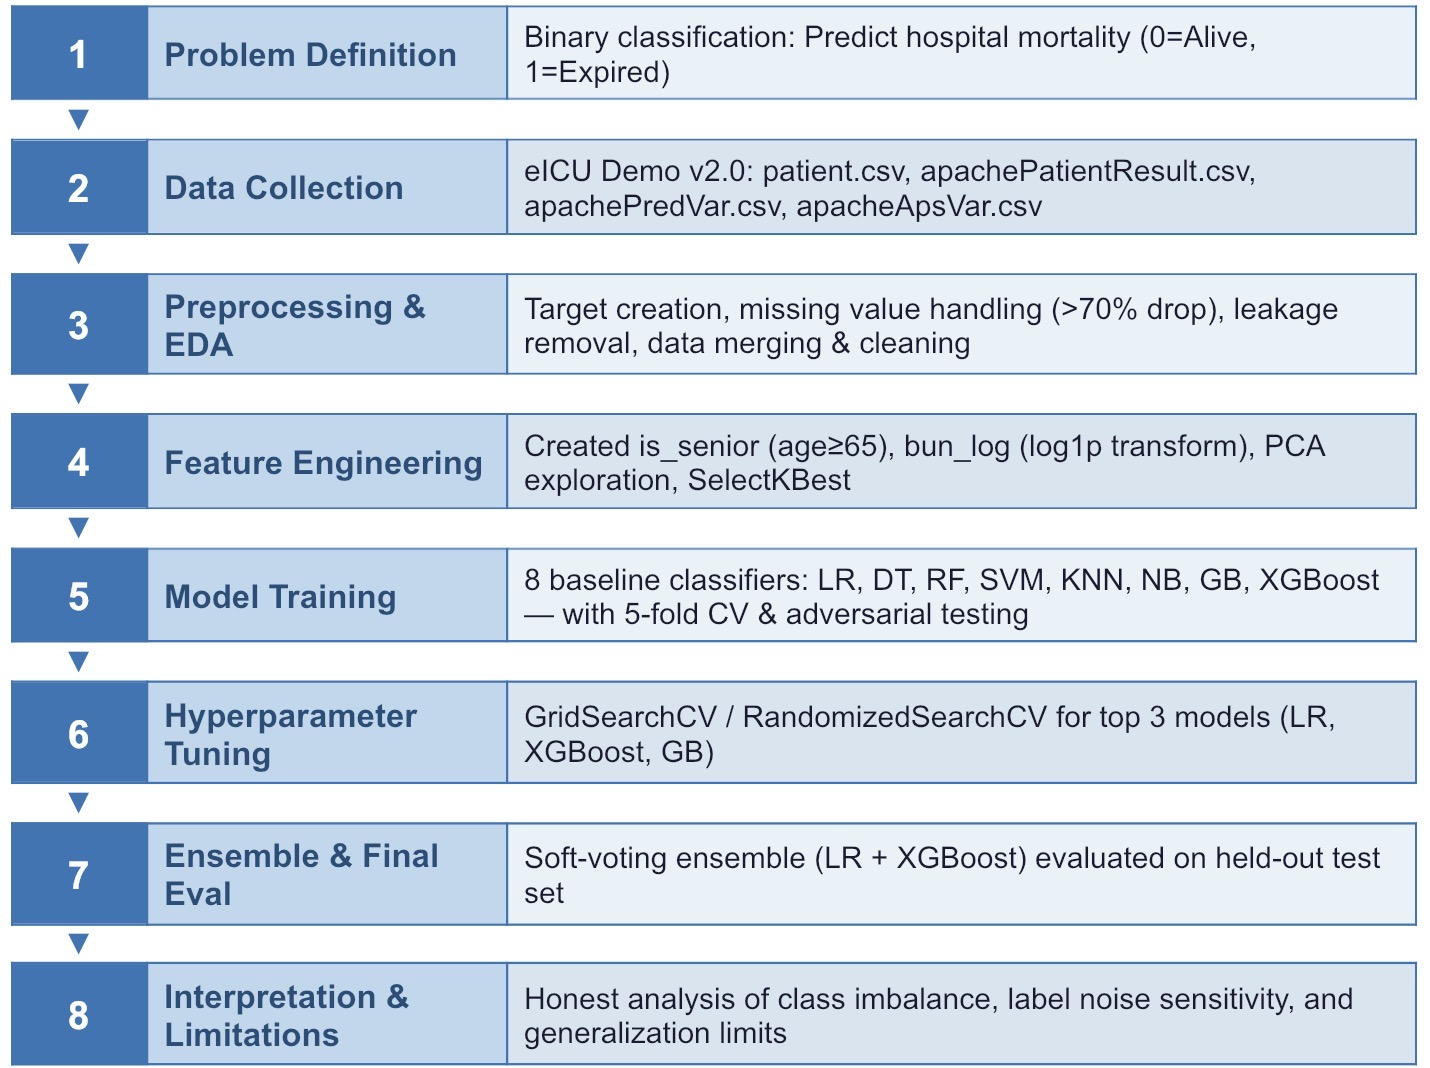
\includegraphics[width=\linewidth]{U.jpeg}
    \caption{Project workflow pipeline showing all stages from data preprocessing to model evaluation.}
    \label{fig:pipeline}
\end{figure}


\section{Introduction and Motivation}

Predicting patient outcomes in intensive care units (ICU) is one of the most important and challenging tasks in clinical medicine. Doctors and nurses working in ICUs need to make fast and reliable decisions, and having tools that can help identify high-risk patients early can significantly improve care and save lives. Machine learning offers a practical way to build such tools by learning patterns from large amounts of patient data.

The motivation for this project comes from the growing availability of structured clinical data and the increasing use of AI in healthcare. The eICU Collaborative Research Database provides a rich source of anonymized ICU patient records from multiple hospitals across the United States. This multi-center nature of the dataset makes it especially interesting because it introduces heterogeneity, meaning that patient populations, data distributions, and clinical practices may vary between hospitals. This makes it a realistic and challenging setting for machine learning.

The goal of this project is to build models that can predict whether an ICU patient will survive or expire during their hospital stay, based on clinical and demographic information available at or shortly after admission. Beyond just building a model that works on a single dataset, the project also investigates how robust these models are when facing realistic challenges such as class imbalance, noisy labels, and heterogeneous data.
The project follows a structured machine learning pipeline, progressing from data preprocessing and feature engineering to model training and evaluation. The final outcome is a voting ensemble model that combines multiple classifiers to achieve more balanced and reliable predictive performance.
The project aims to address the research question: Can machine learning models predict hospital mortality using ICU patient data, and how well do they generalize across heterogeneous patient populations? .

\section{Related Work}

\subsection{Dataset Characteristics and Early Benchmarking Studies
}
The eICU Collaborative Research Database provides a large multi-center dataset containing patient demographics, vital signs, laboratory results, and clinical outcomes. Although the dataset paper itself does not propose specific machine learning models or report evaluation metrics, it outlines essential preprocessing steps such as data cleaning, de-identification, and structured formatting of clinical variables. Its multi-hospital nature makes it particularly suitable for studying heterogeneous patient populations.

Building on this dataset, Sheikhalishahi et al. [1] applied multiple machine learning models, including logistic regression, artificial neural networks (ANN), and Bidirectional Long Short-Term Memory (BiLSTM) networks, to predict mortality and length of stay. Their preprocessing involved separating numerical and categorical variables, applying one-hot encoding and entity embeddings, and using 5-fold cross-validation. The study evaluated performance using AUROC, AUPRC, sensitivity, specificity, mean absolute error (MAE), and R², demonstrating that BiLSTM models outperformed traditional methods due to their ability to capture temporal dependencies.

In addition, a comprehensive review of machine learning in healthcare [3] examined commonly used models such as logistic regression, random forest, and deep learning architectures. The review highlighted preprocessing techniques including handling missing values, feature normalization, and feature selection. Evaluation metrics across studies included accuracy and AUROC, confirming the effectiveness of machine learning approaches in healthcare prediction tasks.



 

\subsection{Explainable and Ensemble Machine Learning Models
}
Recent research has focused on explainable and interpretable machine learning models, which are essential in clinical settings. An explainable ICU mortality prediction study [2] utilized models such as logistic regression, decision trees, and gradient boosting. The preprocessing involved feature selection using the Cox proportional hazards model to reduce dimensionality while maintaining predictive performance. The primary evaluation metric used was AUC-PR, demonstrating that feature selection enhances interpretability without significantly reducing accuracy.

Further advancements are observed in explainable machine learning approaches using XGBoost models [9]. In this work, preprocessing involved feature engineering from time-series data by summarizing variables using statistical measures such as mean and variability over time windows. The model was evaluated using AUROC, average precision, and sensitivity, showing that feature engineering improves both interpretability and predictive performance.

Similarly, another study [8] applied random forest, gradient boosting, and logistic regression models for ICU mortality prediction. The preprocessing included handling missing values and performing feature selection, while evaluation metrics included accuracy, AUROC, and F1-score. The results indicated that ensemble models outperform simpler models.

In the context of septic ICU patients, ensemble learning methods such as random forest, extra trees, and support vector machines (SVM) were applied [10]. The preprocessing involved addressing class imbalance using SMOTE and performing hyperparameter tuning through grid search. The models were evaluated using accuracy, AUROC, sensitivity, specificity, and F1-score, demonstrating that ensemble approaches provide strong and stable predictive performance.



\subsection{Deep Learning and Advanced Clinical Prediction Models
}
Deep learning models have shown strong capability in capturing complex patterns in ICU data. A study using convolutional neural networks (CNNs) [6] applied preprocessing techniques such as time-series feature extraction and handling class imbalance through sampling methods. The model was evaluated using accuracy, root mean square error (RMSE), and R², achieving high predictive performance in mortality and length-of-stay prediction tasks.

More advanced work [7] explored hybrid and ensemble machine learning approaches, combining deep learning and traditional models. The preprocessing included data normalization and feature engineering, while evaluation metrics included AUROC, precision, and recall. The results demonstrated that combining multiple models enhances predictive accuracy and robustness.


 

\subsection{Dataset Shift, Generalization, and Real-World Challenges
}

A key challenge in healthcare machine learning is dataset shift, where differences between training and deployment data reduce model performance. Subbaswamy and Saria [4] analyzed this issue from a theoretical perspective, emphasizing that models must be robust to distributional changes. This study did not focus on specific models, preprocessing, or metrics but highlighted a fundamental limitation in real-world applications.

Generalization across hospitals has also been studied extensively. Zech et al. [5] applied deep learning models and used preprocessing techniques such as data normalization and hospital-based data splitting. Model performance was evaluated using AUROC, and the study showed that models trained on one hospital often perform poorly on others, highlighting generalization challenges in heterogeneous environments.

Temporal dataset shift has also been investigated in recent work [11], where random forest and gradient boosting models were used. The preprocessing involved temporal grouping and feature transformation, while evaluation was conducted using AUROC. The results demonstrated that model performance degrades over time due to changes in data distribution, emphasizing the need for robust and adaptive models.


\section{Data Description and Preprocessing}

\subsection{Dataset}
The dataset used in this project is the eICU Collaborative Research Database (Demo Version 2.0), which contains anonymized ICU patient records collected from multiple hospitals across the United States. This multi-center nature makes it realistic and diverse, covering a wide range of patient demographics, clinical conditions, and outcomes.

Four tables were selected for this project based on their relevance to mortality prediction:

\begin{itemize}
    \item \textbf{patient.csv } demographic and discharge status information (source of the target variable).
    \item \textbf{apachePatientResult.csv } severity scores and outcome-related data (APACHE scoring).
    \item \textbf{apachePredVar.csv } predicted clinical variables from ICU admission.
    \item \textbf{apacheApsVar.csv } physiological measurements collected on admission.
    \end{itemize}
The target variable was derived from the hospitaldischargestatus column in the patient table: 0 for survived and 1 for expired. The class distribution showed a clear imbalance, with approximately 91.6 percent of patients surviving and only 8.4 percent deceased.

\subsection{Exploratory Data Analysis (EDA)
}
Before preprocessing, the data was explored to understand its structure and identify issues. The key findings were:
\begin{itemize}
    \item \textbf{Class Imbalance:} Around 91.6 percent survived and 8.4 percent expired — this guided the choice of evaluation metrics.
.
    \item \textbf{Missing Values:  } Varied across tables. Apache predicted variables had very high missingness; APS variables had none.
    \item \textbf{Numerical Distributions:} APACHE scores were right-skewed with most values in lower ranges.
    \item \textbf{Outliers:  } Present in several features but retained since extreme ICU values often reflect real critical conditions.
    \item \textbf{Correlations:  } APACHE score and Acute Physiology Score were strongly correlated, indicating some redundancy.


    \end{itemize}

\subsection{Preprocessing Steps
} The preprocessing pipeline included several key steps:

\subsubsection{Data Integration:
} All four tables were merged using patientunitstayid as the common key. Since APACHE tables contained multiple rows per patient, they were aggregated first — numerical columns by mean, and the outcome table by keeping the first record per patient. A left join was applied to preserve all patients. After merging, duplicate columns were removed and the dataset was validated to confirm one-row-per-patient format (2520 rows total).

\subsubsection{Missing Value Handling:}
Columns with more than 70 percent missing values were dropped. A relatively high threshold was chosen to avoid losing clinically important features since missing data is common in healthcare. Remaining missing values were kept at this stage and later handled in the preprocessing pipeline using median imputation for numerical features and most-frequent imputation for categorical ones. This was done after the train-test split to prevent data leakage.

\subsubsection{Leakage Removal:
} Several columns containing post-discharge or outcome-related information were identified and removed to prevent data leakage. These included actual discharge status, ICU and hospital length of stay actuals, and predicted mortality scores. These features would not be available at prediction time and must be excluded.

\subsubsection{Transformation Pipeline:
} A scikit-learn ColumnTransformer pipeline was defined to handle preprocessing consistently during training. Numerical features were imputed with the median and scaled using StandardScaler. Categorical features were imputed with the most frequent value and encoded using OneHotEncoder. This pipeline was applied inside each model pipeline to avoid any leakage.



\section{Methodology}

\subsection{Feature Engineering
} Two new features were created based on clinical relevance:
\begin{itemize}
    \item \textbf{is-senior:} A binary feature indicating whether the patient is 65 or older (1) or not (0). Age is a well-known risk factor for ICU mortality and this simplification captures the clinical threshold.
    \item \textbf{bun-log: } A log-transformed version of blood urea nitrogen (BUN) using log1p to reduce skewness and handle near-zero values safely.

   
    \end{itemize}
PCA was applied to the numeric feature space for exploration only and was not included in the final training pipeline. SelectKBest with mutual information was also tested as a feature selection step in one candidate pipeline.

\subsection{Model Selection
} Eight classification algorithms were trained and compared as baselines:
\begin{itemize}
    \item \textbf{Logistic Regression:} (C=1, solver=liblinear, class-weight=balanced).

    \item \textbf{Decision Tree:} (class-weight=balanced)

    \item \textbf{Random Forest:} (class-weight=balanced)

    \item \textbf{SVM:}  (probability=True, kernel=rbf, class-weight=balanced)

    \item \textbf{K-Nearest Neighbors:} default setting.
    \item \textbf{Naive Bayes: }(GaussianNB)
    \item \textbf{Gradient Boosting:}  (n-estimators=100, random-state=42)

    \item \textbf{XGBoost} (scale-pos-weight to handle imbalance, n-estimators=200, learning-rate=0.05, max-depth=3)
 
    \end{itemize}
    
 \subsection{Training Strategy
} The data was split into three parts:
\begin{itemize}
    \item \textbf{} 80 percent training set / 20 percent test set (first split, stratified)
    \item \textbf{} Training set further split into 80 percent  final train / 20 percent validation (second split, stratified)
    \item \textbf{} 5-fold stratified cross-validation used to evaluate model stability

    \end{itemize}
To simulate real-world data quality issues, adversarial conditions were introduced by randomly flipping 10 percent of training labels (161 samples). Models were retrained on these noisy labels and compared against the clean baseline to measure robustness.

\subsection{Hyperparameter Tuning
} The top three candidate models — Logistic Regression, XGBoost, and Gradient Boosting — were selected for hyperparameter tuning based on baseline performance. GridSearchCV was used for Logistic Regression and SVM, while RandomizedSearchCV (n-iter=12) was used for tree-based models to reduce computation time. All searches used 5-fold stratified cross-validation with F1-score as the optimization metric.
\subsection{Ensemble} A soft-voting ensemble was built by combining the tuned Logistic Regression and tuned XGBoost models. Soft voting uses predicted probabilities rather than hard class labels, which generally produces better results when models are well-calibrated. The ensemble was evaluated on the validation set before final testing.


\section{Experimental Results and Discussion
}
\subsection{Baseline Model Performance} All eight models were trained on the final training set and evaluated on the validation set. Since the dataset is imbalanced, the focus was on F1-score, recall, and AUC-ROC rather than accuracy. The key results were:
\begin{itemize}
    \item \textbf{} XGBoost achieved the highest baseline F1-score (0.328947) and AUC-ROC (0.799732), making it the strongest baseline model.

    \item \textbf{} Logistic Regression was the second-best model and provided a useful interpretable alternative.

    \item \textbf{} Models like KNN, Naive Bayes, and Decision Tree showed weaker minority-class detection.


    \end{itemize}
Cross-validation further confirmed that Logistic Regression and XGBoost were the most consistent models across folds, while KNN and Random Forest struggled with the minority class.

\subsection{Adversarial Testing
} When models were retrained using the noisy labels (10 percent flipped), performance dropped across the board. Precision and F1-score decreased, and AUC-ROC values were lower than in the clean baseline setting. Some models showed higher recall under noise, but this came at the cost of more false positives and lower precision. This confirms that data quality is a critical factor — even moderate mislabeling can meaningfully reduce model reliability in clinical prediction.
\subsection{Hyperparameter Tuning Results
} After tuning, XGBoost remained the strongest individual model. However, the improvement over baseline was modest, suggesting that the baseline configuration already captured most of the learnable signal. Gradient Boosting and Logistic Regression also improved slightly but not dramatically. This indicates that the dataset itself, rather than tuning, limits further performance gains.

\subsection{Final Test Set Results
} The final evaluation was performed once on the held-out test set. The table below summarizes the performance of all final candidate models:

\begin{figure}[t]
    \centering
    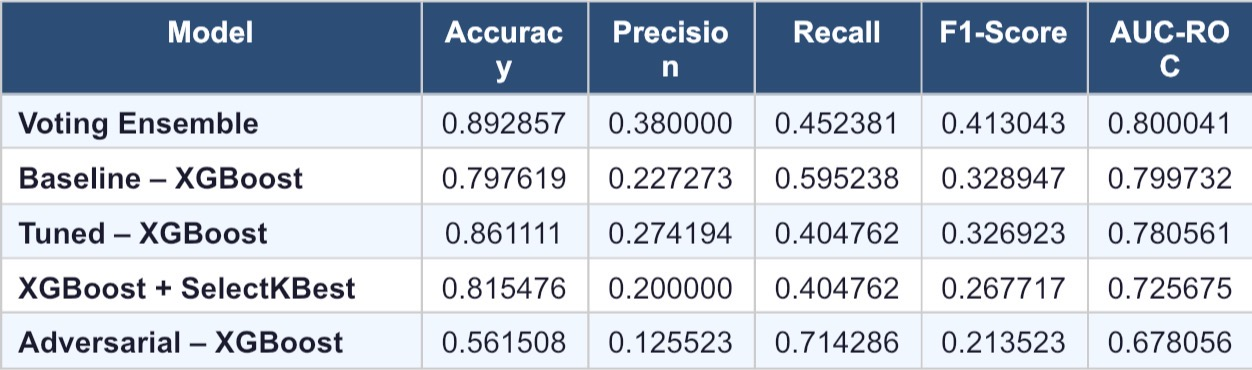
\includegraphics[width=\linewidth]{K.jpeg}
    \caption{
}
    \label{fig:pipeline}
\end{figure}
\subsection{Discussion of Results
}
\subsubsection{Voting Ensemble — Best Overall Performance
}
On the held-out test set, the Voting Ensemble achieved the best overall performance, with the highest F1-score of 0.413043 and the highest AUC-ROC of 0.800041. It also achieved the highest accuracy (0.892857) among all models.
In terms of class-specific performance, the ensemble reached a precision of 0.380000 and recall of 0.452381, indicating a balanced ability to correctly identify mortality cases while controlling false positives. Compared to individual models, the ensemble improved the trade-off between precision and recall, leading to the strongest F1-score. This confirms that combining models (Logistic Regression and XGBoost) enhances robustness and overall predictive performance.


\subsubsection{XGBoost — Strong Individual Baseline
}
The baseline XGBoost model demonstrated strong performance with an AUC-ROC of 0.799732, which is very close to the ensemble model. Notably, it achieved the highest recall (0.595238) among all models, meaning it was the most effective at identifying true mortality cases. However, this came at the cost of low precision (0.227273), indicating a higher number of false positives.
The tuned XGBoost model improved accuracy (0.861111) and precision (0.274194) compared to the baseline, but recall decreased to 0.404762, resulting in a slightly lower F1-score (0.326923) and AUC-ROC (0.780561). This suggests that hyperparameter tuning shifted the model toward a more conservative prediction strategy, improving precision but reducing its ability to detect mortality cases.

\subsubsection{XGBoost with SelectKBest — Feature Reduction Impact
}
The feature selection approach using SelectKBest resulted in lower performance, with an F1-score of 0.267717 and AUC-ROC of 0.725675. Although recall (0.404762) remained comparable to the tuned model, precision dropped to 0.200000, indicating weaker discrimination between classes.
This suggests that reducing the feature set removed important predictive information rather than eliminating noise. The results indicate that ICU mortality prediction benefits from a richer feature space, where multiple variables contribute to model performance.

\subsubsection{Adversarial XGBoost — Impact of Label Noise
}

The adversarial XGBoost model, trained with 10 percent label noise, showed a significant decline in overall performance. While it achieved a high recall (0.714286), its precision dropped to 0.125523, resulting in a low F1-score (0.213523) and reduced AUC-ROC (0.678056).
This indicates that the model became highly sensitive but unreliable, predicting many false positives. The results clearly demonstrate that label noise negatively affects model reliability, which is particularly critical in healthcare applications where data quality directly impacts decision-making.

\subsubsection{Interpretation of F1-Score
}

The best-performing model achieved an F1-score of approximately 0.41, which may appear moderate compared to results on balanced datasets. However, this is a realistic and meaningful outcome for ICU mortality prediction.
The dataset is highly imbalanced, with mortality cases representing a small minority of patients. In such scenarios, optimizing both precision and recall simultaneously is challenging. Increasing recall (detecting more true mortality cases) often leads to lower precision (more false positives), and vice versa.
The Voting Ensemble successfully achieved the best balance between these competing objectives, improving over all individual models. This indicates that the model provides meaningful predictive performance under realistic clinical conditions, where both sensitivity and reliability are essential.

\subsection{Visualizations}
Final confusion matrices and ROC curves were generated for all five candidate models on the test set to provide a clear and comprehensive visual confirmation of the numerical results obtained. These visualizations help illustrate how each model performs in distinguishing between classes, offering additional insight beyond the reported evaluation metrics. 

\subsubsection{Confusion matrices: }
Generated using sns.heatmap with the Blues colormap, annotated with the count of true positives, false positives, true negatives, and false negatives for each model. The matrices made it visually clear which models were better at detecting the minority class versus which ones defaulted to predicting survival for most patients.

\subsubsection{ROC curves: }
Plotted for all five candidates on the test set using the plot-roc-curves function. The AUC-ROC value was shown in the legend for each model. The ensemble curve consistently ran above the individual model curves at most threshold levels, visually confirming its superior discrimination ability.

\begin{figure}[t]
    \centering
    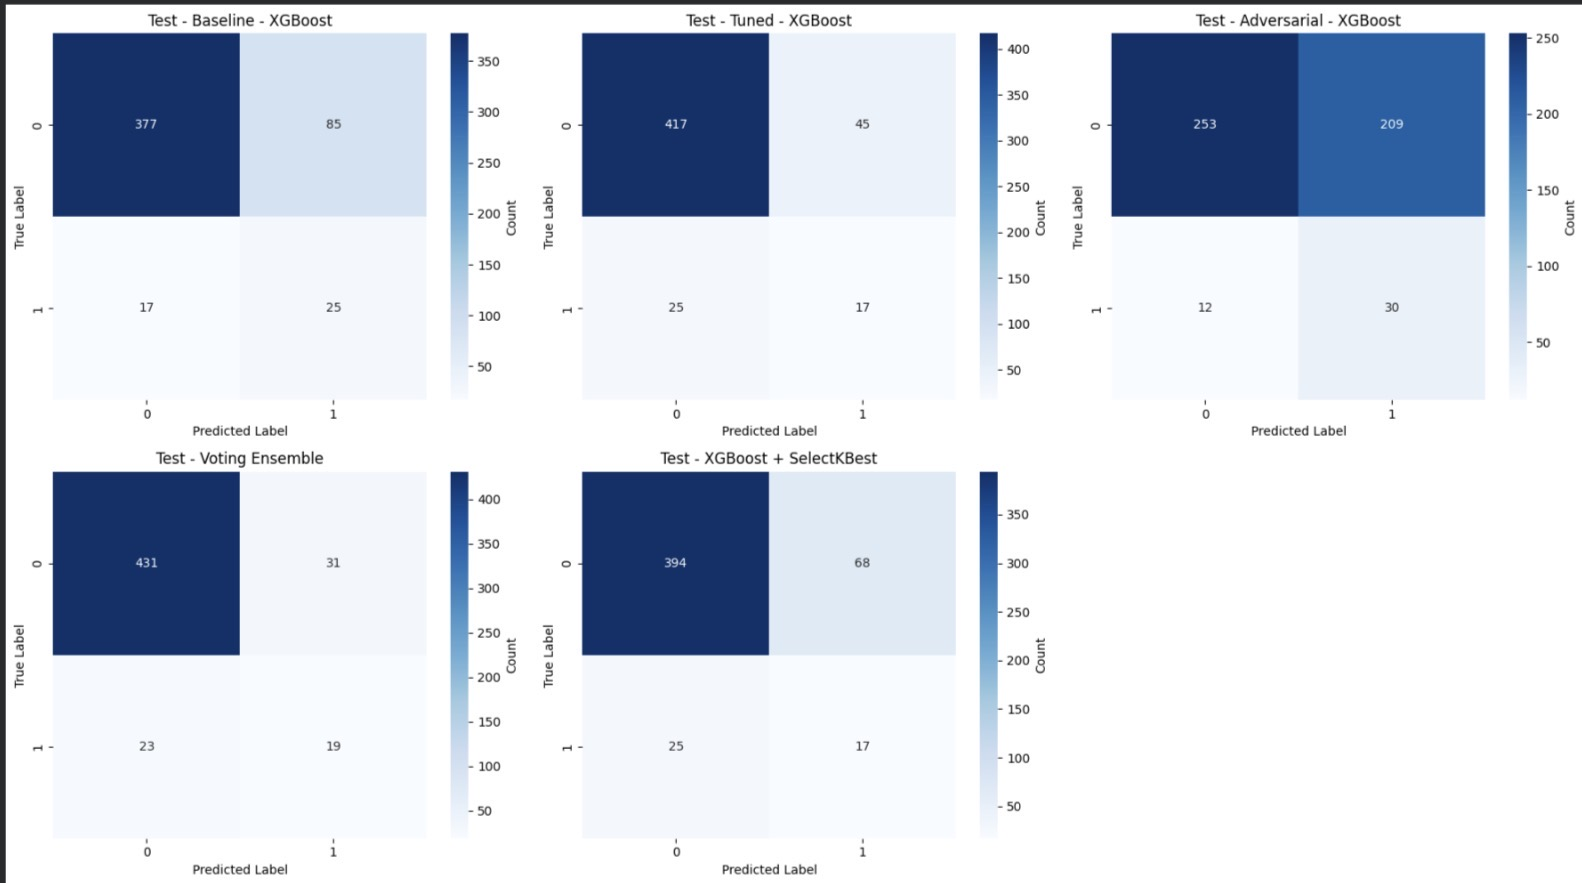
\includegraphics[width=\linewidth]{C.jpeg}
    \caption{
}
    \label{fig:pipeline}
\end{figure}

\begin{figure}[t]
    \centering
    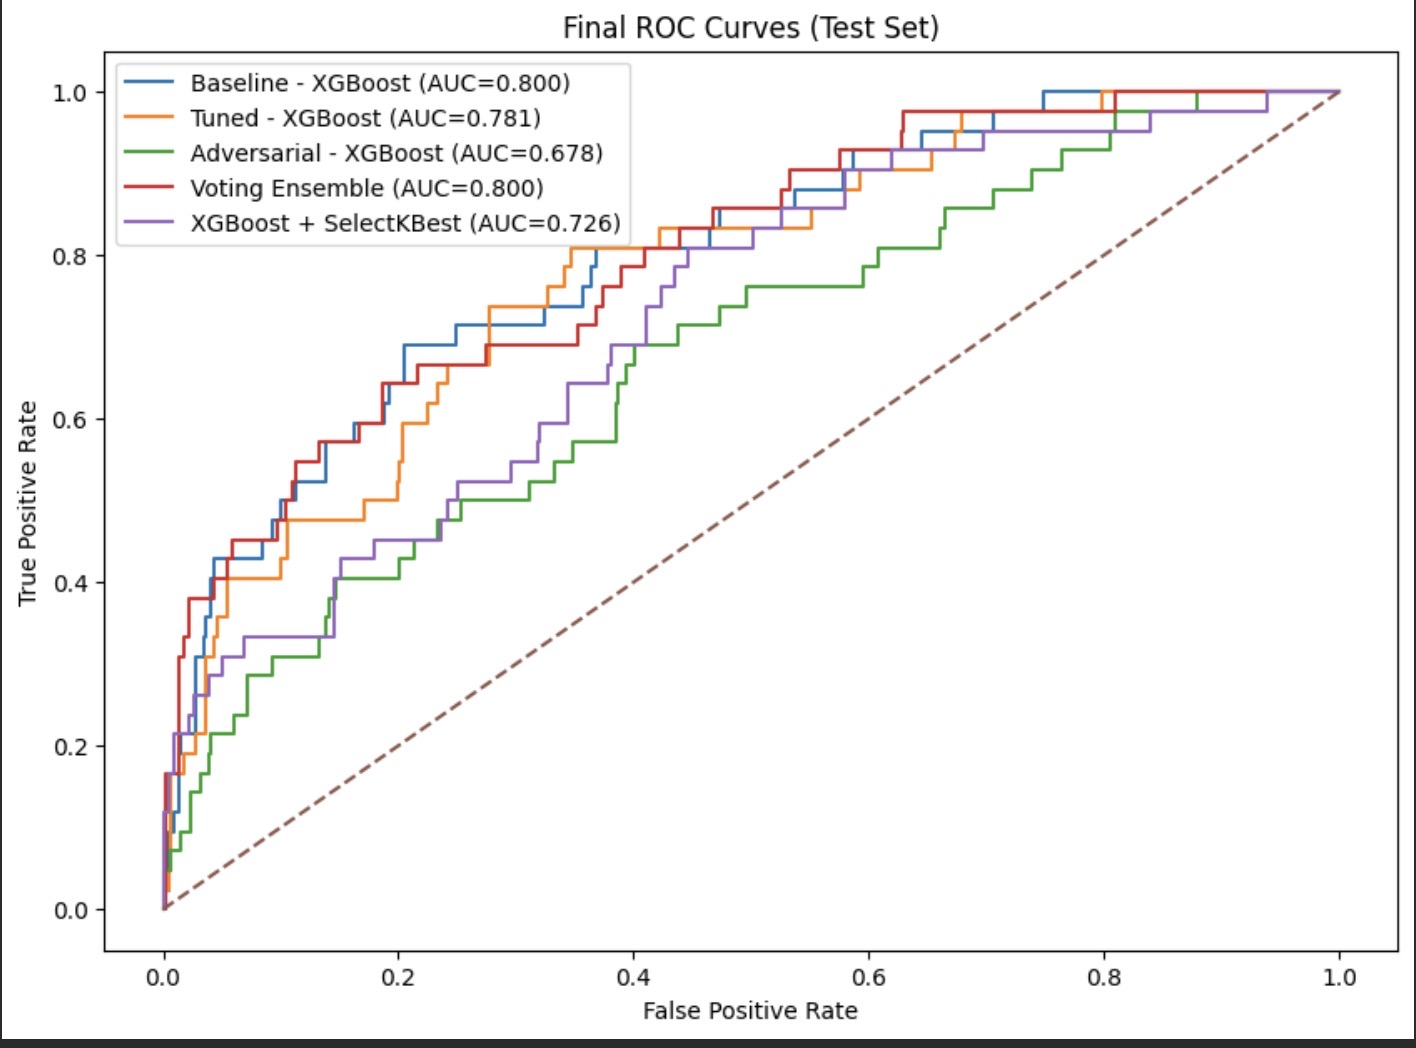
\includegraphics[width=\linewidth]{R.jpeg}
    \caption{
}
    \label{fig:pipeline}
\end{figure}
\section{Conclusion and Future Work
} 
\subsection{Conclusion} This project developed and evaluated machine learning models for ICU mortality prediction using the eICU Collaborative Research Database. The work followed a complete end-to-end pipeline, including careful preprocessing, feature engineering, multi-model training, hyperparameter tuning, and adversarial robustness analysis.

The main findings are:
\begin{itemize}
    \item \textbf{} XGBoost was the strongest individual model, with an AUC-ROC of 0.799 at baseline.

    \item \textbf{} A soft-voting ensemble of Logistic Regression and XGBoost achieved the best final result (F1=0.413, AUC-ROC=0.800).

    \item \textbf{} Class imbalance is a major challenge — evaluation metrics beyond accuracy are essential.

    \item \textbf{} Label noise had a meaningful negative impact, showing that model robustness needs more attention in clinical settings.

    \item \textbf{} Hyperparameter tuning alone provided limited gains over well-configured baselines.
    
    \end{itemize}
Overall, the project demonstrates that machine learning can provide useful predictive support for ICU mortality, while also showing that real-world deployment would require stronger validation, better robustness guarantees, and clinical interpretability tools.

\subsection{Limitations}
Several honest limitations were identified:
\begin{itemize}
    \item \textbf{} The models were trained and tested on a single dataset from a limited demo version — external validation on larger or different hospital populations was not done.

    \item \textbf{} Time-series clinical variables (e.g., trends in vital signs over the ICU stay) were not used, which limits how well the model captures patient deterioration.

    \item \textbf{} Class imbalance was partially addressed through class weighting, but more advanced strategies like SMOTE or focal loss were not tested.

    \item \textbf{} Explainability (e.g., SHAP values) was not fully implemented, making it harder to justify predictions to clinicians.

    \end{itemize}

\subsection{Future Work
}
Based on the limitations, several directions could improve this work:
\begin{itemize}
    \item \textbf{} Validate models on external hospital datasets or larger eICU versions to assess cross-site generalization.

    \item \textbf{} Incorporate time-series ICU monitoring data using recurrent or temporal models (e.g., LSTM, Transformer).

    \item \textbf{} Apply SMOTE or cost-sensitive learning to better handle class imbalance and improve minority-class detection.

    \item \textbf{} Use SHAP or LIME to produce clinician-friendly explanations of individual predictions.

    \item \textbf{} Systematically optimize classification thresholds for deployment-focused precision-recall tradeoffs.

    \end{itemize}

\section{Github repository link}
https://github.com/Hams770/Health-Risk-Prediction-ML.git

\begin{thebibliography}{99}

\bibitem{ref1}
Sheikhalishahi, S., Balaraman, V., \& Osmani, V. (2020).
Benchmarking machine learning models on multi-centre eICU critical care dataset.
\textit{PLOS ONE}.
\url{https://journals.plos.org/plosone/article?id=10.1371/journal.pone.0235424}

\bibitem{ref2}
Machine learning in healthcare: Review and applications. (2022).
\textit{Physiological Reviews}.
\url{https://journals.physiology.org/doi/10.1152/physrev.00033.2022}

\bibitem{ref3}
Explainable machine learning prediction of ICU mortality. (2021).
\textit{Journal of Biomedical Informatics}.
\url{https://www.sciencedirect.com/science/article/pii/S2352914821001593}

\bibitem{ref4}
Subbaswamy, A., \& Saria, S. (2020).
From development to deployment: Dataset shift, causality, and shift-stable models in health AI.
\textit{Biostatistics}, 21(2), 345--361.
\url{https://academic.oup.com/biostatistics/article/21/2/345/5613899}

\bibitem{ref5}
Zech, J. R., Badgeley, M. A., Liu, M., Costa, A. B., Titano, J. J., \& Oermann, E. K. (2018).
Variable generalization performance of a deep learning model across hospitals.
\textit{PLOS Medicine}.
\url{https://journals.plos.org/plosmedicine/article?id=10.1371/journal.pmed.1002683}

\bibitem{ref6}
Deep learning approach for ICU mortality and length of stay prediction. (2023).
\textit{Journal of Biomedical Informatics}.
\url{https://www.sciencedirect.com/science/article/pii/S1532046423002472}

\bibitem{ref7}
Advanced machine learning for clinical prediction. (2025).
\textit{npj Digital Medicine}.
\url{https://www.nature.com/articles/s41746-025-02114-y}

\bibitem{ref8}
Machine learning models for ICU mortality prediction. (2025).
\textit{PMC}.
\url{https://pmc.ncbi.nlm.nih.gov/articles/PMC12975804/}

\bibitem{ref9}
Explainable machine learning for ICU mortality prediction. (2025).
\textit{Scientific Reports}.
\url{https://www.nature.com/articles/s41598-025-13299-3}

\bibitem{ref10}
Machine learning for mortality prediction in septic ICU patients. (2025).
\textit{Journal of Clinical Medicine}.
\url{https://www.mdpi.com/2077-0383/14/10/3495}

\bibitem{ref11}
Temporal dataset shift in ICU data and its impact on model performance. (2025).
\textit{ScienceDirect}.
\url{https://www.sciencedirect.com/science/article/pii/S229196942500287X}

\bibitem{ref12}
Johnson, A., Pollard, T., Badawi, O., \& Raffa, J. (2019).
eICU Collaborative Research Database Demo (version 2.0).
\textit{PhysioNet}.
\url{https://physionet.org/content/eicu-crd-demo/2.0.1/}

\end{thebibliography}




\end{document}
